\documentclass[a4paper, 11pt]{article}
\usepackage{listings}
\usepackage{graphicx}
\usepackage{mathtools}
\graphicspath{ {./plots/} }

\lstset{basicstyle=\tiny\ttfamily,breaklines=true}
\lstset{frame=Trbl,numbers=left}

\title{Humble Introduction to Linear Regression in Julia Programming }
\author{Júlio César de Brito Gardona}
\date{January 13, 2023}

\begin{document}


\maketitle

\tableofcontents
\addtocontents{toc}{\protect\rule{\textwidth}{.2pt}\par}
\pagebreak

\section{Linear Regression}
Linear regression analysis is used to \textit{predict the value} of a variable based on the value of another variable. The variable you want to predict is called the \textit{dependent variable}. The variable you are using to predict the other variable's value is called the \textit{independent variable}.

This form of analysis estimates the coefficients of the linear equation, involving one or more independent variables that best predict the value of the dependent variable. Linear regression fits a straight line or surface that minimizes the discrepancies between predicted and actual output values. There are simple linear regression calculators that use a \textbf{least squares} method to discover the best-fit line for a set of paired data. You then estimate the value of X (dependent variable) from Y (independent variable).

\section{Simple Linear Regression using GLM}
\textbf{GLM} is a library that helps build linear and generalized linear models in Julia. The objective of this section is to demonstrate how to use linear regression to find a solution for a linear problem. Later in this article, we will be implementing all solutions from scratch using \textbf{Julia Programming}. We will study the relationship between the age of a dog and the number of veterinary visits it had. In a fabricated sample we have 10 random dogs. Lets plot the dataset below and observe.

\begin{figure}[ht]
\caption{Dog data in a scatter plot (x, y values)}
\label{fig:dgdata}
\centering
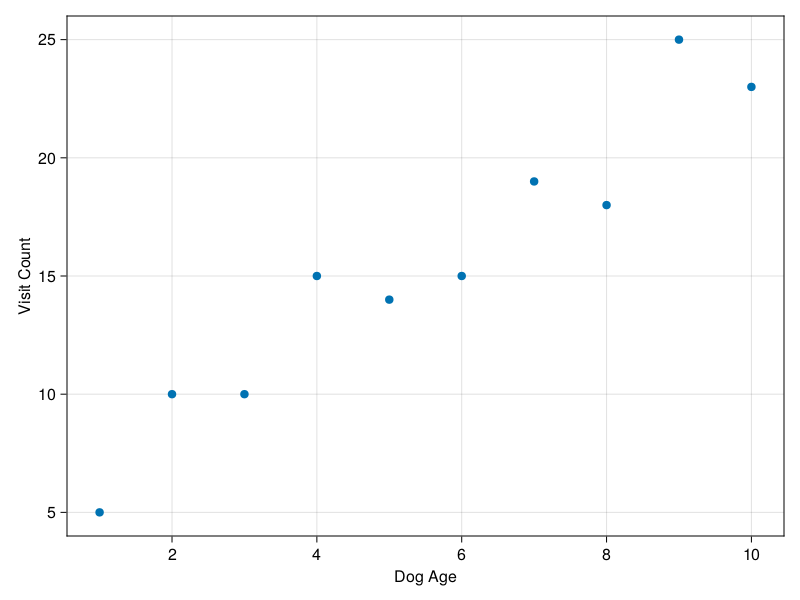
\includegraphics[width=.5\textwidth]{dogdata}
\end{figure}

We clearly see there is a linear correlation here in figure \ref{fig:dgdata}, meaning when one of these variables increase or decrease, the other increases or decreases in a roughly proportional amount.

Linear regression will allow us to make predictions on data we had not seen before. We do not have a dog in sample that is 8.5 year old, but its possible to look in the regression's line and estimate the dog will have 21 veterinary visits in its life. We can analyse variables for possible relationships and hypothesize that correlate variables are casual to one another.

First we import data from this CSV in github as shown in listing~\ref{slinreg}. We build a DataFrame with $x, y$ data, that will be used in linear model lm. After fit our model, we extract m and b coefficients, build our predictions and plot all data and line shown figure~\ref{fig:linearreg}.

\begin{lstlisting}[caption={Simple Linear Regression},label=slinreg]
using GLM, DataFrames, CairoMakie, Statistics, CSV, Distributions;

data = CSV.read(download("https://bit.ly/3goOAnt"), DataFrame);

ols = lm(@formula(y ~ x), data);
@info ols;

b, m = coef(ols);

fig = Figure();

ax, s = scatter(fig[1, 1], data.x, data.y);
ax.xlabel = "Dog Age";
ax.ylabel = "Visit Count";

l = lines!(ax, data.x, m*data.x .+ b, color=:red);
Legend(fig[1, 2],[s, l], ["Data", "Predictions"]);

fig
\end{lstlisting}


\begin{figure}[ht]
\caption{Linear regression in dog data }
\label{fig:linearreg}
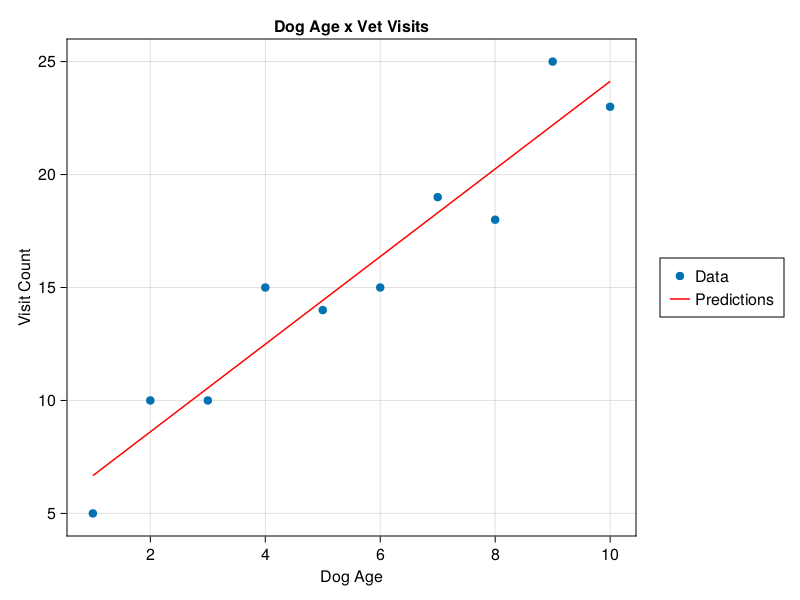
\includegraphics[width=.5\textwidth]{glmlinearr}
\centering
\end{figure}

All we have did was using the package GLM, and in the next sections we will learn a bunch of theory on how to fit this line from scratch.

\section{Residuals and Squared Errors}
How statistics tools like GLM can calculates a line that fits to these points? A few questions comes in mind:

\begin{description}
	\item[What defines a best fit?] The answer is pretty simple. We minimize the squares, or more specifically the sum of the residuals. If we draw any line through the points, the residual will be the numeric difference between the line and the points.
	
	Points above the line will have a positive residual, and points below the line a negative residual. It is the subtracted difference between predicted y-values(derived from the line) and the actual y-values (which came from the data). Another name for residuals are errors, because they reflect how wrong our line is in predicting the data. In listing~\ref{lst:residuals} we calculate the residuals.

\begin{lstlisting}[caption={Calculating the residuals for a given line and data},label={lst:residuals}]
data = CSV.read(download("https://bit.ly/3goOAnt"), DataFrame);

# fit a model from csv data
model = lm(@formula(y ~ x), data);

# get the m(x) and b(intercept) coefficients
b, m = coef(model);

# calc the residuals by hand from m and b coefficients
points = Tuple.(eachrow(data));
println("m: $m, b: $b");

for p in points
    yactual = p[2];
    ypredicted = m * p[1] + b;
    residual = yactual - ypredicted;
    println("residual -> $residual");
end

Out:
m: 4.733333333333331, b: 1.93939393939394
residual -> -1.6727272727272702
residual -> 1.3878787878787904  
residual -> -0.5515151515151508 
residual -> 2.5090909090909097  
residual -> -0.43030303030302974
residual -> -1.369696969696971  
residual -> 0.6909090909090878  
residual -> -2.24848484848485   
residual -> 2.812121212121209   
residual -> -1.1272727272727288 
\end{lstlisting}

	If we are fitting a straight line through our 10 data points, we likely want to minimize these residuals in total so there is the least gap possible between the line and the points. We need calculate the total using the \textit{sum of squares}, which simply square each residual and sum them as shown in listing~\ref{lst:sumsq}.
	
\begin{lstlisting}[caption={Calculating the sum of squares for a given line and data},label={lst:sumsq}]
data = CSV.read(download("https://bit.ly/3goOAnt"), DataFrame);
describe(data)

# fit a model from csv data
model = lm(@formula(y ~ x), data)

# get the m(x) and b(intercept) coefficients
b, m = coef(model)

# calc the residuals by hand from m and b coefficients
points = Tuple.(eachrow(data));
println("m: $m, b: $b");

sumofsquares = 0;

for p in points
    yactual = p[2];
    ypredicted = m * p[1] + b;
    residual = yactual - ypredicted;
    sumofsquares += residual^2;
    println("residual -> $residual");
end

println("sum of squared errors: $sumofsquares");

Out:
m: 4.733333333333331, b: 1.93939393939394
residual -> -1.6727272727272702
residual -> 1.3878787878787904  
residual -> -0.5515151515151508 
residual -> 2.5090909090909097  
residual -> -0.43030303030302974
residual -> -1.369696969696971  
residual -> 0.6909090909090878  
residual -> -2.24848484848485   
residual -> 2.812121212121209   
residual -> -1.1272727272727288 

sum of squared errors: 28.096969696969683
\end{lstlisting}	
	 
	\item[How do we get to that best fit?] We'll see in next section how to optimize and produce a minimum sum of squares.
	
\end{description}

\section{Finding the Best Line Fit}

Now we have a way to measure the quality of the line against the data: \textbf{the sum of squares}. The lower we can make this number, the better the fit.

There are a couple of search algorithm we can employ, which try to find the right set of values to solve a given problem. We can use \textit{closed form, matrix inversion, matrix decomposition, gradient descent, and stochastic gradient descent}. This is the most important thing when we are dealing with \textbf{"training" of a machine learning algorithm}. So, when we "train" a machine learning model, we really are minimizing a loss function.
\subsection{Closed Form}

For a simple linear regression with only one input and output variable we'll be using the \textit{closed form equations} to calculate m and b coefficients as shown in listing~\ref{lst:cfeq}.
\begin{equation}
\begin{aligned}
m = \frac{n\sum xy - \sum x \sum y}{n\sum x^2 - (\sum x)^2}\\[10pt]
b = \frac{\sum y}{n} -m\frac{\sum x}{n}
\end{aligned}
\end{equation}

\begin{lstlisting}[caption={Calculating m and b using closed form equations for simple linear regressions},label={lst:cfeq}]

data = CSV.read(download("https://bit.ly/3goOAnt"), DataFrame);

points = Tuple.(eachrow(data));
n = length(points);

m = (n * sum(p[1] * p[2] for p in points) - sum(p[1] for p in points) * sum(p[2] for p in points)) /
    (n * sum(p[1]^2 for p in points) - sum(p[1] for p in points)^2);

b = (sum(p[2] for p in points) / n) - (m * (sum(p[1] for p in points) / n));

println("m: $m, b: $b");

Out:

m: 1.9393939393939394, b: 4.7333333333333325

\end{lstlisting}

We are seeing the importance of linear algebra and calculus in machine learning. We'll be using a lot concepts through this tutorial.

\subsection{Inverse Matrix Techniques}
We can transposed and inverse matrices to fit linear regression. We calculate the vector of coefficients $b$ using a given matrix of input variable values $X$ and a vector of output variables values $y$ as below.

$$
b = (X^{T} * X)^{-1}*X^{T}*y
$$

\begin{lstlisting}[label={lst:inmat},caption={Using inverse and transposed matrices to fit a linear regression}]
data = CSV.read(download("https://bit.ly/3goOAnt"), DataFrame);

# Extract input variables (all rows, all columns but last column
x = data.x;

# Add a placeholder "1" column to generate the intercept
x1 = [x ones(length(x))];
y = data.y;

# Calculate coefficients for slope and intercept
b = inv(x1' * x1) * x1'*y;
println("m: $(b[1]), b: $(b[2])");

Out:

m: 1.9393939393939412, b: 4.733333333333334
\end{lstlisting}

We have to stack a column of 1s next to our $X$ column. This will generate the intercept $\beta_0$ coefficient. Since this column is all 1s, it effectively generates the intercept and not just a slope $\beta_1$.

A better choice, if our dataset have a lot of data with lots of dimensions is use \textbf{Matrix Decomposition}, also a trick we learned in linear algebra class. In this specific case, we take our matrix $X$, append an additional column of 1s to generate the intercept $\beta_0$ just like before, and then decompose it into two component matrices $Q$ and $R$:

$$
X = Q * R
$$

Here is how we use $Q$ and $R$ to find the beta coefficient in the matrix form $b$:
$$
b = (R^{-1}*Q^T)*y
$$

We show how to calculate the coefficients using QR decomposition in listing~\ref{lst:qrdecomp}.

\begin{lstlisting}[label={lst:qrdecomp},caption={Calculate coefficients for slope and intercept using QR decomposition}]
using Random, CSV, DataFrames, GLM, Plots, LinearAlgebra;

data = CSV.read(download("https://bit.ly/3goOAnt"), DataFrame);

# Extrac input variables (all rows, all columns but last column)
x = data.x;
# Add placeholder "1" column to generate intercept
x1 = [x ones(length(x))];

y = data.y;

# Calculate coefficients for slope and intercept using QR decomposition
Q, R = qr(x1);
b = (inv(R) * Q') * y;

println("m: $(b[1]), b: $(b[2])");

Out:

m: 1.9393939393939394, b: 4.733333333333333
\end{lstlisting}

\subsection{Gradient Descent}
\textit{Gradient Descent} is an optimization algorithm that uses derivatives and iterations to minimize/maximize a set of parameters against an objective. We'll do a simple experiment in a quadratic function $f(x) = (x - 3)^2 + 4$ to understand how Gradient Descent works.

Basically, this algorithm works trying to find the smallest slope in a function curve. The bigger the curve slope, bigger is the step, and smaller steps for smaller slopes, until the slope is flat, a value of 0. As told before, Gradient Descent will try to get the smallest slope in function presented before, using its derivative:
$$
\frac{d}{dx} = 2(x -3)
$$

We can see the results of gradient descent algorithm in figure~\ref{fig:rgdesc}, where we have the function in blue line and the smalles slope represented as a orange diamond marker. The code is shown in listing~\ref{lst:graddesc}.

\begin{figure}[ht]
\caption{The results of Gradient Descent on $f(x) = (x - 3)^2 + 4$}
\label{fig:rgdesc}
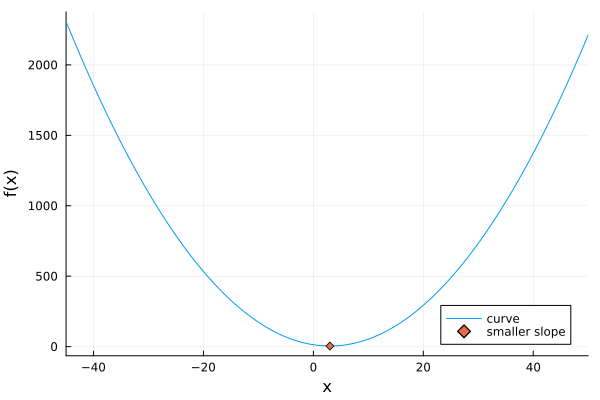
\includegraphics[width=.5\textwidth]{gradientdescent}
\centering
\end{figure}

\begin{lstlisting}[label={lst:graddesc},caption={Gradient Descent on $f(x) = (x - 3)^2 + 4$}]
using DataFrames, Plots, CSV, GLM, Statistics;

f(x) = (x - 3)^2 + 4;
df(x) = 2(x - 3);

# the learning rate
L = 0.0001;

# the number of iterations
iterations = 100_000;

# start at random x
x = rand(-15:15);

for i in 1:iterations
	# get the actual slope
	slope = df(x);
	# update x by subtracting the lernin rate * slope
	x -= L * slope;
end
println("x: $x, f(x): $(f(x))");

plot(f, xlims=(-45, 50), label="curve", xlabel="x", ylabel="f(x)");
scatter!([x], [f(x)], label="smaller slope", m=:diamond);

Out:

x: 2.9999999732585456, f(x): 4.000000000000001
\end{lstlisting}

Now, back to linear regression context, we'll be using \textit{Gradient Descent} to optimize our loss function, that is, the \textbf{sum of squares}, so we need to find the derivatives of our sum of squares function with respect to $m$ and $b$, or $\beta_0$ and $\beta_1$. In mathematical notation, $e(x)$ represents our sum of squares loss function, and below, we have our partial derivatives. The algorithm implementation is shown in listing~\ref{lst:graddescmb}. 

\begin{equation}
\begin{aligned}
e(x)=\sum_{i=0}^{n} ((mx_i + b) -y_i)^2 \\[5pt]
\frac{d}{dm}e(x)=\sum_{i=0}^{n}2(b+mx_i - y_i)x_i \\[5pt]
\frac{d}{db}e(x)=\sum_{i=0}^{n}(2b+2mx_i -2y_i)
\end{aligned}
\end{equation}

\begin{lstlisting}[label={lst:graddescmb},caption={Gradient Descent and Linear Regression}]
using DataFrames, Plots, CSV, GLM, Statistics;

points = Tuple.(eachrow(data));

m = 0.0;
b = 0.0;
iterations = 100_000;
L = 0.0001;

for i in 1:iterations
	# slope with respect to m
	dm = sum(2*(b + m * p[1] - p[2]) * p[1] for p in points);
	db = sum(2 * b + 2 * m * p[1] - 2 * p[2] for p in points);
	m -= L * dm;
	b -= L * db;
end

println("m: $m, b: $b");

Out:

m: 1.9393939393940933, b: 4.733333333332265
\end{lstlisting}

\subsection{Stochastic Gradient Descent}
In real world, is unlikely we train our model in all training data as we did earlier. In practice, we'll perform in only one sample of the dataset in each iteration. There are some benefits as reduce computational significantly, as each iteration does not have to traverse the entire training dataset but only part of it. Another benefit is reduce overfitting. Exposing the training algorithm to only part of the data on each iteration keeps changing the loss landscape so it doesn't settle in the loss minimum.

\begin{lstlisting}[label={lst:stochgdesc},caption={Stochastic Gradient Descent and Linear Regression}]
data = CSV.read(download("https://bit.ly/2KF29Bd"), DataFrame);

x = data.x;
y = data.y;

n = nrow(data);
m, b = 0.0, 0.0;
samplesize = 1;
L = .0001;
epochs = 1_000_000;

for i in 1:epochs
	index = sample(1:n, samplesize, replace=false);
	xsample = x[index];
	ysample = y[index];

	ypred = m * xsample .+ b;
	dm = (-2 / samplesize) .* sum(xsample .* (ysample - ypred));
	db = (-2 / samplesize) .* sum(ysample - ypred);
		
	m -= L * dm;
	b -= L * db;
	if i % 100000 == 0
		println("$i, m: $m, b: $b");
	end
end
		
println("y = $(m)x + $b");

Out:

100000, m: 1.9579158289625898, b: 4.674668871028908
200000, m: 1.9065866808529823, b: 4.740743049961377
300000, m: 1.9388175332832558, b: 4.729718715915005
400000, m: 1.890698414725821, b: 4.773847087545454
500000, m: 1.960409987067053, b: 4.75671097560848
600000, m: 1.9512744265749982, b: 4.7147132450763145
700000, m: 1.958477280864674, b: 4.724809006902896
800000, m: 1.934422524146756, b: 4.741838282895306
900000, m: 1.9619442123795858, b: 4.7105226993781475
1000000, m: 1.947817988669668, b: 4.7136572583933
y = 1.947817988669668x + 4.7136572583933
\end{lstlisting}

\section{The Correlation Coefficient}
If data is extremely spread out, its going to drive up the variance to the point of predictions become less accurate and useful, resulting in large residuals. The under fitting is also going to undermine our predictions because the data is so spread out. We need numerically measure how "off" our predictions are. We'll use the \textit{correlation coefficient}, also called \textit{Pearson correlation}, which measures the strength of the of the relationship between two variables as a value between -1 and 1. A correlation coefficient closer to 0 indicates there is no correlation. A correlation coefficient closer to 1 indicates a \textbf{strong positive}, correlation, meaning when a variable increases, another also increases. If its closer to -1, then it indicates a \textbf{strong negative} correlation, which means as one variable increases the other proportionally decreases. The correlation coefficient is denoted by $r$. Since its closer than 0, more spread is the data, and has little correlation. Below we have an example of how to calculate the correlation coefficient in listing~\ref{lst:corrcoff}.

\begin{lstlisting}[label={lst:corrcoff},caption={The Correlation Coefficient calculated with standard library function}]
data = CSV.read(download("https://bit.ly/2KF29Bd"), DataFrame);

cor(data.x, data.y)

Out:

0.9575860952087217
\end{lstlisting}

\subsection{Calculating the Correlation Coefficient}

\begin{equation}
r =\frac{n\sum xy - (\sum x)(\sum y)}{\sqrt{n \sum x^2 - (\sum x)^2} \sqrt{n \sum y^2 - (\sum y)^2}}
\end{equation}

\begin{lstlisting}[label={lst:corrcoeffhand},caption={Calculating the Correlation Coefficient}]
data = CSV.read(download("https://bit.ly/2KF29Bd"), DataFrame);
points = Tuple.(eachrow(data));
n = length(points);

numerator = n * sum(p[1] * p[2] for p in points) - (sum(p[1] for p in points) * sum(p[2] for p in points));

denominator = sqrt(n * sum(p[1]^2 for p in points) - sum(p[1] for p in points)^2) * sqrt(n * sum(p[2]^2 for p in points) - sum(p[2] for p in points)^2);
coeff = numerator / denominator;
println(coeff);

Out:

0.9575860952087218
\end{lstlisting}

\section{Statistical Significance}
Is it possible I see a linear relationship in my data due to random chance? How can we be 95\% sure the correlation between these variables is significant and do not coincidental? We'll use hypothesis test, because we need not just express correlation, but also quantify how confident we are that correlation coefficient did not occur by chance. Let's pursue our hypothesis test with 95\% confidence using a two-tailed test, exploring if there is a relationship between this two variables.

\begin{equation}
\begin{aligned}
H_0:\rho=0(implies\ no\ relationship) \\[5pt]
H_1:\rho \neq 0(relationship\ is\ present)
\end{aligned}
\end{equation}

We use the T-distribution rather than a normal distribution to do hypothesis testing with linear regression. The dataset has 10 records in our sample and therefore we have 9 degrees of freedom($10 - 1 = 9$).

\begin{lstlisting}[label={lst:cvalue},caption={Calculating the critical value from a T-distribution}]
n = 10;

lowercv = quantile(TDist(n - 1), .025);
uppercv = quantile(TDist(n - 1), .975);
println("uppercv: $uppercv, lowercv: $lowercv");

Out:

uppercv: 2.2621571627982044, lowercv: -2.262157162798205

\end{lstlisting}

The critical value is $\pm2.262$ and we calculated this in Julia as shown in Listing~\ref{lst:cvalue}. If our test value happens to fall outside this range, then we can reject our null hypothesis. To calculate the test value $t$, we need to use the following formula. Again $r$ is the correlation coefficient and $n$ is the sample size:

\begin{equation}
\begin{aligned}
t = \frac{r}{\sqrt{\frac{1-r^2}{n - 2}}} \\[5pt]
\end{aligned}
\end{equation}

Let's solve the test in Julia. If our test value falls outside the critical range of 95\% confidence, we accept that our correlation is not by chance.

The test value is approximately 9.39956, which is definitely outside our range $\pm2.262$ so we can reject our null hypothesis and say our correlation is real. That's because the p-value is remarkably significant: 0.000005976. This is well below our .05 threshold as shown in Listing~\ref{lst:sign}.

\begin{lstlisting}[label={lst:sign},caption={Testing significance for linear-looking data}]
n = 10;
lowercv = quantile(TDist(n - 1), .025);
uppercv = quantile(TDist(n - 1), .975);
println("uppercv: $uppercv, lowercv: $lowercv");

r = 0.957586;
testvalue = r / sqrt((1-r^2) / (n-2));
println("the test value (t) is: $testvalue");

# calculate the p-value
pvalue = 1.0 - cdf(TDist(n - 1), testvalue);
# two-tailed, so multiply by 2
pvalue *= 2;
println("p-value for t > 0 is: $pvalue");

Out:

uppercv: 2.2621571627982044, lowercv: -2.262157162798205
the test value (t) is: 9.399564671312076
p-value for t > 0 is: 5.9763860877914965e-6
\end{lstlisting}

\section{Coefficient of Determination ($r^2$)}

The coefficient of determination, called $r^2$, measures how much variation in one variable is explained by the variation of other variable. It's also the square of the correlation coefficient $r$. As $r$ approaches a perfect correlation (-1 or 1), $r^2$ approaches 1. Essentially, $r^2$ shows how much two variables interact with each other. The Listing~\ref{lst:coeffdet} shows how to calculate $r^2$.

A coefficient of determination of 0.916971 is interpreted as 91.6971\% of
the variation in x is explained by y (and vice versa), and the remaining
8.3029\% is noise caused by other uncaptured variables; 0.916971 is a pretty
good coefficient of determination, showing that x and y explain each other's
variance. But there could be other variables at play making up that
remaining 0.083029

\begin{lstlisting}[caption={Creating a correlation matrix and squaring it},label={lst:coeffdet}]
df = CSV.read(download("https://bit.ly/2KF29Bd"), DataFrame);
coeffdet = cor(df.x, df.y)^2;
println(coeffdet);

Out:

0.916971129737087
\end{lstlisting}

\section{Standard Error of the Estimate}

One way to measure the overall error of a linear regression is the SSE, or
sum of squared error. We learned about this earlier where we squared each
residual and summed them. If $\hat{y}$ (pronounced "y-hat") is each predicted
value from the line and $y$ represents each actual y-value from the data, here
is the calculation:
$$
SSE = \sum(y - \hat{y})^2
$$

However, all of these squared values are hard to interpret so we can use
some square root logic to scale things back into their original units. We will
also average all of them, and this is what the standard error of the estimate (
$Se$) does. If $n$ is the number of data points, Listing~\ref{lst:se} shows how we
calculate the standard error $Se$ in Julia.

$$
Se=\sqrt{\frac{\sum(y - \hat{y})^2}{n - 2}}
$$

\begin{lstlisting}[caption={Calculating the Standard Error of Estimate},label={lst:se}]
df = CSV.read(download("https://bit.ly/2KF29Bd"), DataFrame);
points = Tuple.(eachrow(df))

n = length(points);

# Regression line
m = 1.939;
b = 4.733;

se = sqrt(sum((p[2] - (m * p[1] + b))^2 for p in points) / (n - 2));
println("Se: $se");

Out:

Se: 1.87406793500129
\end{lstlisting}

\section{Prediction Intervals}

With a linear regression, we hope that data follows a normal distribution in a linear fashion. A regression line serves as the shifting "mean" of our bell curve, and the spread of the data around the line reflects the variance/standard deviation.

When we have a normal distribution following a linear regression line, we
have not just one variable but a second one steering a distribution as well.
There is a confidence interval around each y prediction, and this is known
as a \textit{prediction interval}. With our veterinary example, estimating the
age of a dog and number of vet visits, I want to know the prediction interval
for number of vet visits with 95\% confidence for a dog that is 8.5 years old. We are 95\% confident that an 8.5 year old dog will have between 16.462 and 25.966 veterinary visits.

\begin{lstlisting}[caption={Calculating a prediction interval of vet visits for a dog that's 8.5 years old},label={lst:predint}]

points = Tuple.(eachrow(data));
n = length(points);

# Linear Regression Line
m = 1.939;
b = 4.733;

# calculate prediction interval for x = 8.5
x0 = 8.5;
xmean = sum(p[1] for p in points) / n;
println("xmean: $xmean");

tvalue = quantile(TDist(n - 2), .975);
se = sqrt(sum((p[2] - (m * p[1] +b))^2 for p in points) / (n- 2));

marginoferror = tvalue * se * sqrt(1 + (1 / n) + (n * (x0 -xmean)^2) / (n * sum(p[1]^2 for p in points) - sum(p[1] for p in points)^2));

ypredicted = m * x0 + b;
	
println(ypredicted - marginoferror, ", ", ypredicted + marginoferror);

Out:

xmean: 5.5
16.46251687560351, 25.966483124396493

\end{lstlisting}

\section{Train/Tests Splits}

A basic technique machine learning practitioners use to mitigate overfitting is a practice called the train/test split, where typically 1/3 of the data is set aside for testing and the other 2/3 is used for training (other ratios can be used as well). The training dataset is used to fit the linear regression, while the testing dataset is used to measure the linear regression's performance on data it has not seen before. This technique is generally used for all supervised machine learning, including logistic regression and neural networks. The function below splits and shuffles a dataset, based in a given ratio.

\begin{lstlisting}[caption={Splitting a dataset in a given ratio}]
data = CSV.read(download("https://bit.ly/2KF29Bd"), DataFrame);

function splitdf(df, pct)
    @assert 0 <= pct <= 1
    ids = collect(axes(df, 1))
    shuffle!(ids)
    sel = ids .<= nrow(df) .* pct
    return view(df, sel, :), view(df, .!sel, :);
end

train, test = splitdf(data, .7);
println("Test:", nrow(test), ", Train:", nrow(train));

Out:

Test:3, Train:7
\end{lstlisting}

\end{document}

